\chapter*{Sommario}
\label{cha:sommario}
\addcontentsline{toc}{chapter}{Sommario}

%%%%%%%%%%%%%%%%%%%%%%%%%%%%%%%%%%%%%%%%%%%%%%%%%%%%%%%%%%%%%%%%%%%%%%%%%%
%%%%%%%%%%%%%%%%%%%%%%%%%%%%%%%%%%%%%%%%%%%%%%%%%%%%%%%%%%%%%%%%%%%%%%%%%%
%% Nota
%%%%%%%%%%%%%%%%%%%%%%%%%%%%%%%%%%%%%%%%%%%%%%%%%%%%%%%%%%%%%%%%%%%%%%%%%%
%% Sommario e' un breve riassunto del lavoro svolto dove si descrive
%% l’obiettivo, l’oggetto della tesi, le metodologie e
%% le tecniche usate, i dati elaborati e la spiegazione delle conclusioni
%% alle quali siete arrivati.
%% Il sommario dell’elaborato consiste al massimo di 3 pagine e deve contenere le seguenti informazioni:
%%   contesto e motivazioni
%%   breve riassunto del problema affrontato
%%   tecniche utilizzate e/o sviluppate
%%   risultati raggiunti, sottolineando il contributo personale del laureando/a
%%%%%%%%%%%%%%%%%%%%%%%%%%%%%%%%%%%%%%%%%%%%%%%%%%%%%%%%%%%%%%%%%%%%%%%%%%
%%%%%%%%%%%%%%%%%%%%%%%%%%%%%%%%%%%%%%%%%%%%%%%%%%%%%%%%%%%%%%%%%%%%%%%%%%
Sempre di più la tecnologia si sta diffondendo in ogni aspetto delle nostre vite,
in particolare tra le nuove generazioni di ragazzi che, nati in un mondo già
digitalizzato, hanno avuto un approccio molto più naturale e immediato rispetto alle
generazioni precedenti. Con la continua espansione dei videogiochi, anche la tecnologia
si sta espandendo verso nuove opportunità di intrattenimento, in particolare
spicca tra queste la realtà virtuale come dispositivo emergente.

\section*{La realtà virtuale}
\label{sec:la-realta-virtuale}

Alla base della realtà virtuale ci sono i visori, dispositivi in grado di
immergere l'utente in un mondo virtuale, permettendogli di interagire con esso.

I primi esempi di visore in commercio erano molto semplici come il Google Cardboard,
ovvero una particolare struttura in cartone attraverso la quale era possibile
trasformare uno smartphone in un visore rudimentale, che offriva all'utente la sola
possibilità di orientare lo sguardo nelle tre dimensioni.

Con l'evoluzione delle tecnologie, si sono sviluppate apparecchiature sempre più
complesse che sfruttando diverse innovazioni hanno permesso la cattura di
maggiori interazioni, come il rilevamento della posizione degli arti e la possibilità
di inviare comandi trasformabili in azioni.

Oggi i principali visori si dividono in due categorie: i visori \textit{tethered},
che necessitano di un collegamento ad un computer per funzionare, e i visori \textit{standalone},
che hanno la possibilità di essere utilizzati in maniera autonoma. Tra i visori
più venduti ci sono:

\begin{itemize}
  \item \textbf{Meta Quest 3}: visore standalone alimentato a batteria. Grazie
    alle telecamere presenti sulla struttura del visore, è in grado di rilevare l'orientamento
    della testa, la posizione delle mani e la posizione dei controller, permettendo
    all'utente di interagire con il mondo virtuale senza la necessità di installare
    sensori esterni.

  \item \textbf{HTC Vive Pro}: visore tethered che necessita di un computer per funzionare.
    È uno dei visori più utilizzati nella realtà virtuale in quanto permette di
    avere una maggiore qualità grafica rispetto ai visori indipendenti. È dotato
    di sensori esterni che rilevano la posizione dell'utente nello spazio,
    permettendo una maggiore precisione e una maggiore libertà di movimento. È compatibile
    con molti dispositivi di input oltre ai controller standard, permettendo di
    rilevare anche la posizione di diverse articolazioni o oggetti.
\end{itemize}

\begin{figure}[h!]
  \centering
  \begin{minipage}{0.3\textwidth} % Prima immagine
    \centering
    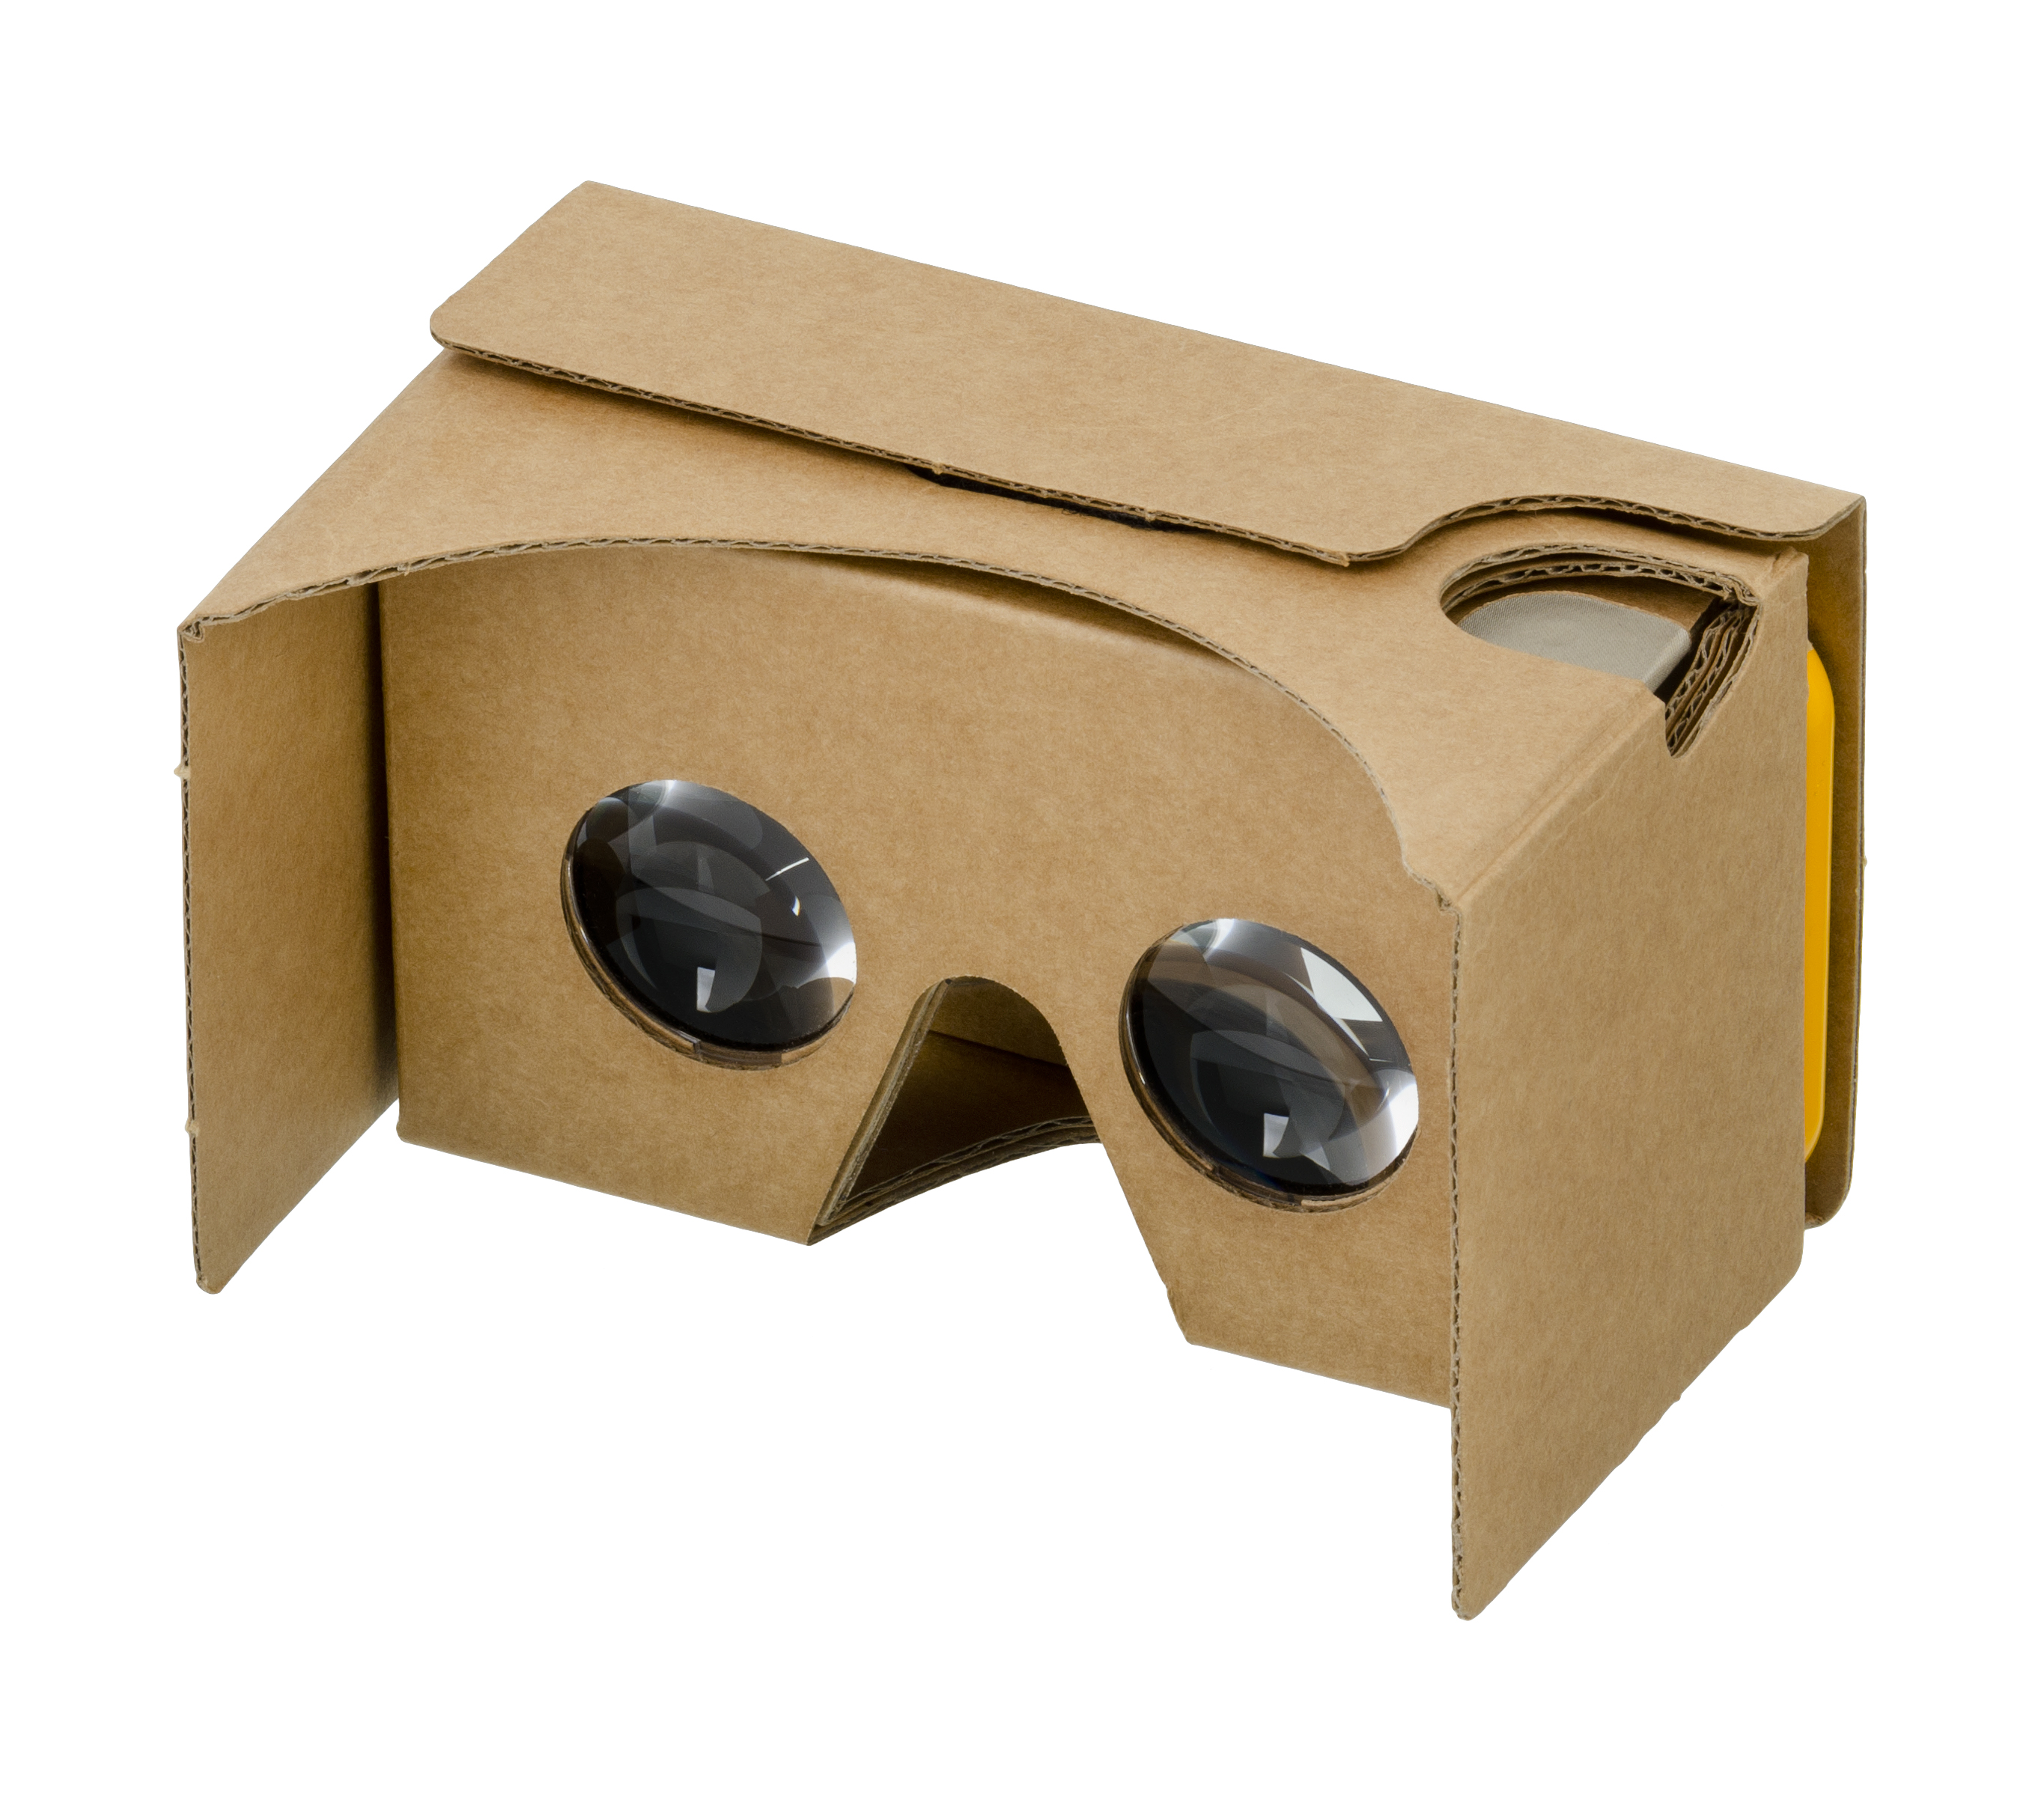
\includegraphics[height=2cm]{images/GoogleCardboard.jpg} % Altezza uniforme
    \caption{Google Cardboard}
    \label{fig:googlecardboard}
  \end{minipage}
  \hfill
  \begin{minipage}{0.3\textwidth} % Seconda immagine
    \centering
    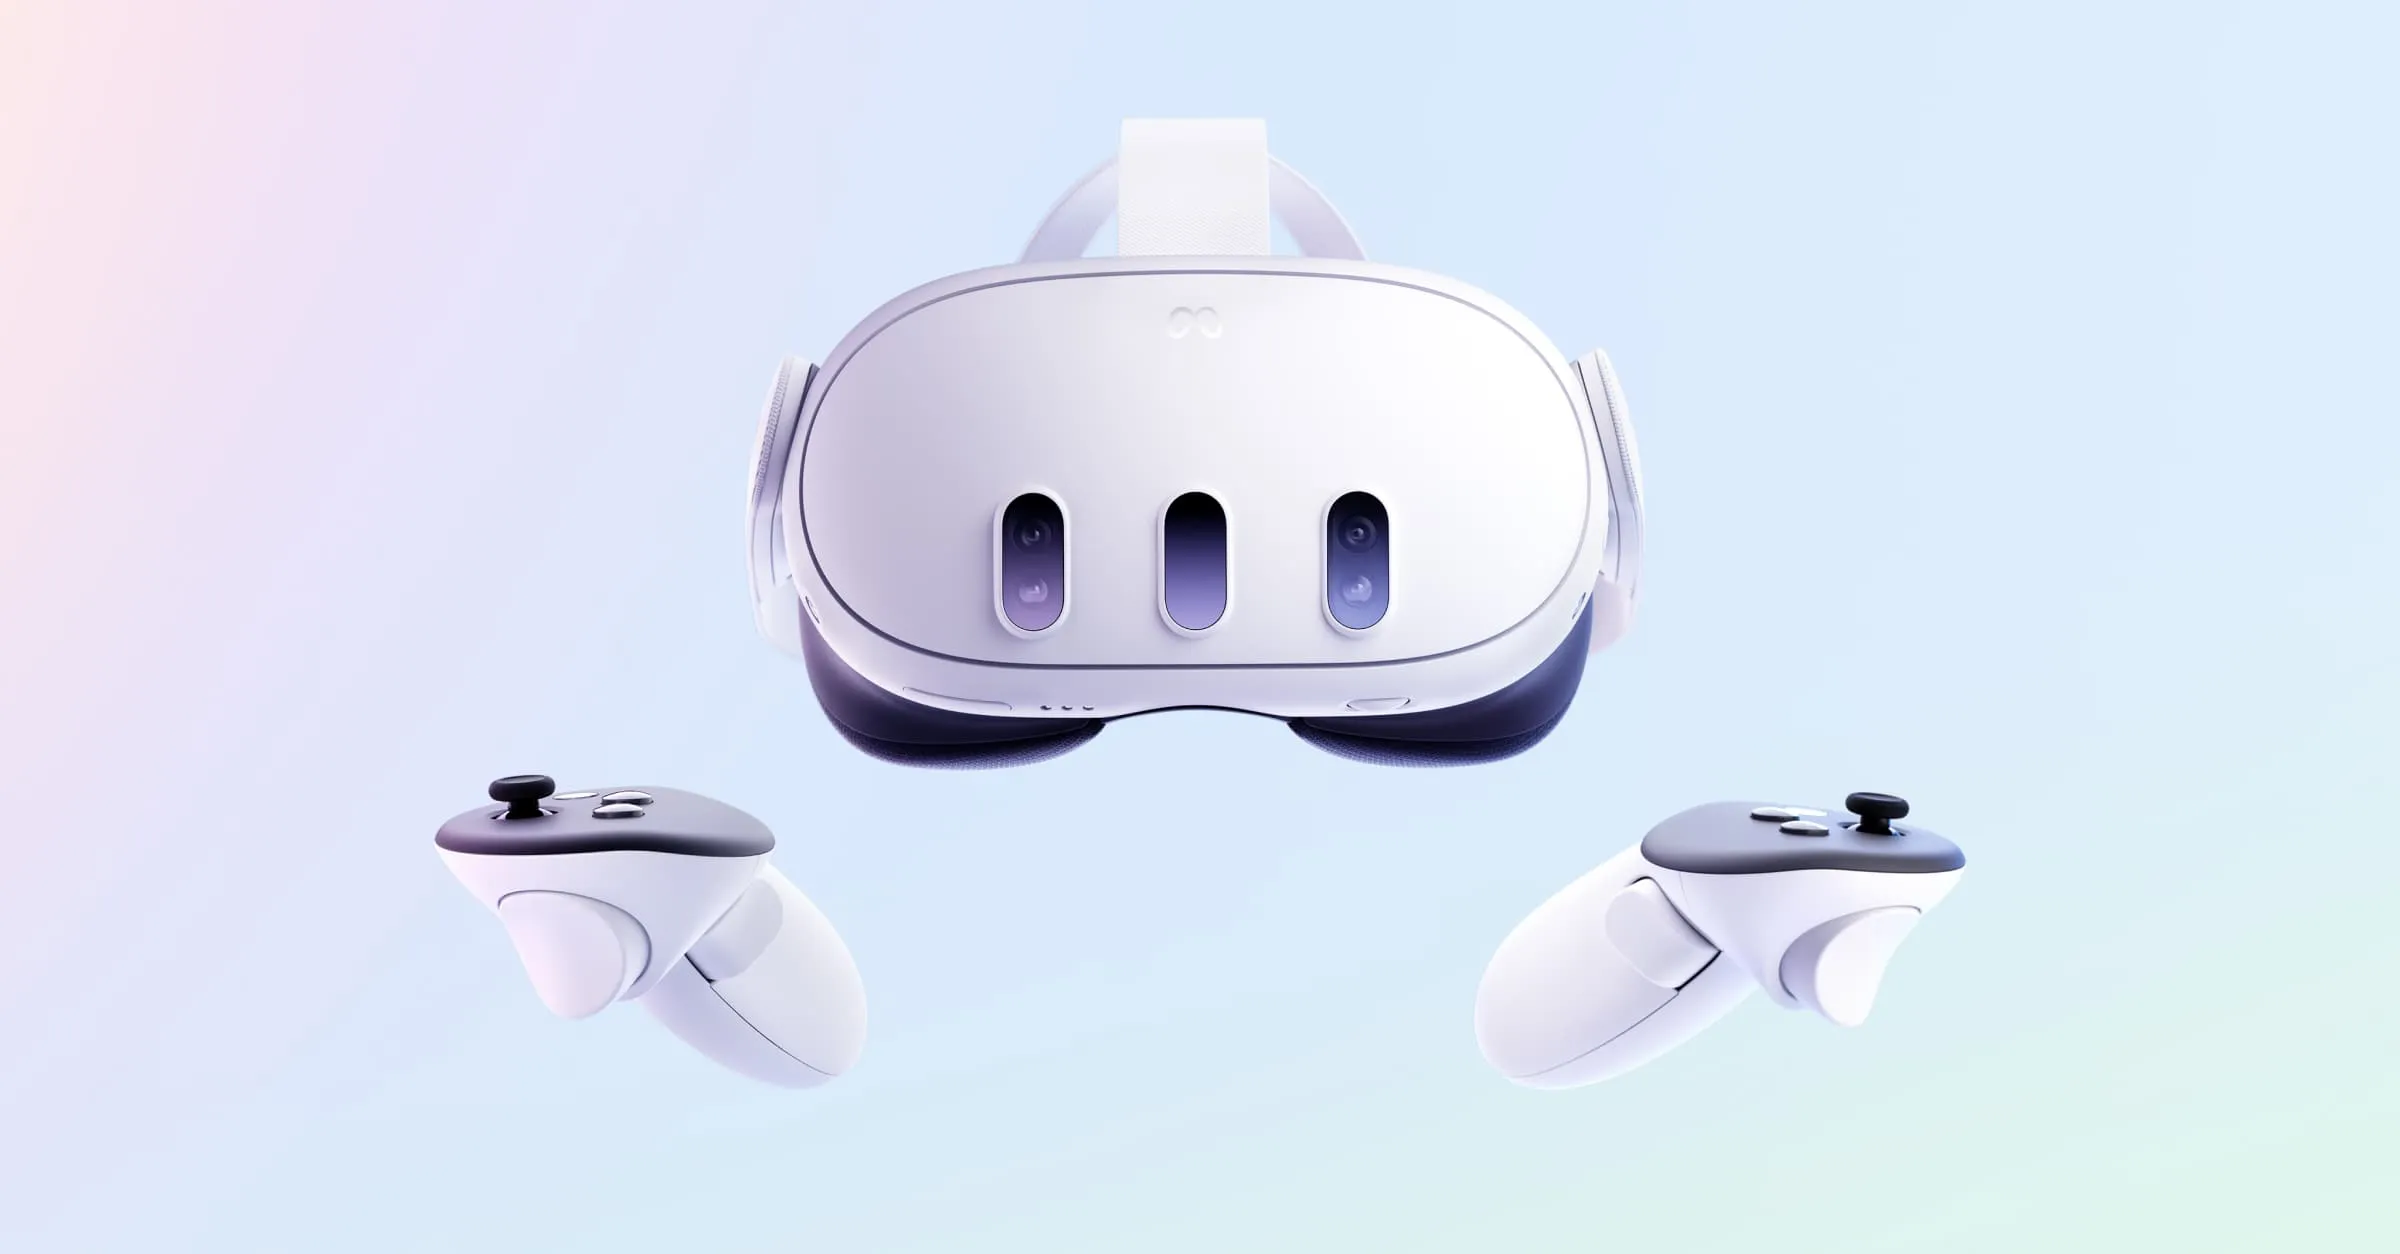
\includegraphics[height=2cm]{images/Quest3.png} % Altezza uniforme
    \caption{Meta Quest 3}
    \label{fig:quest3}
  \end{minipage}
  \hfill
  \begin{minipage}{0.3\textwidth} % Terza immagine
    \centering
    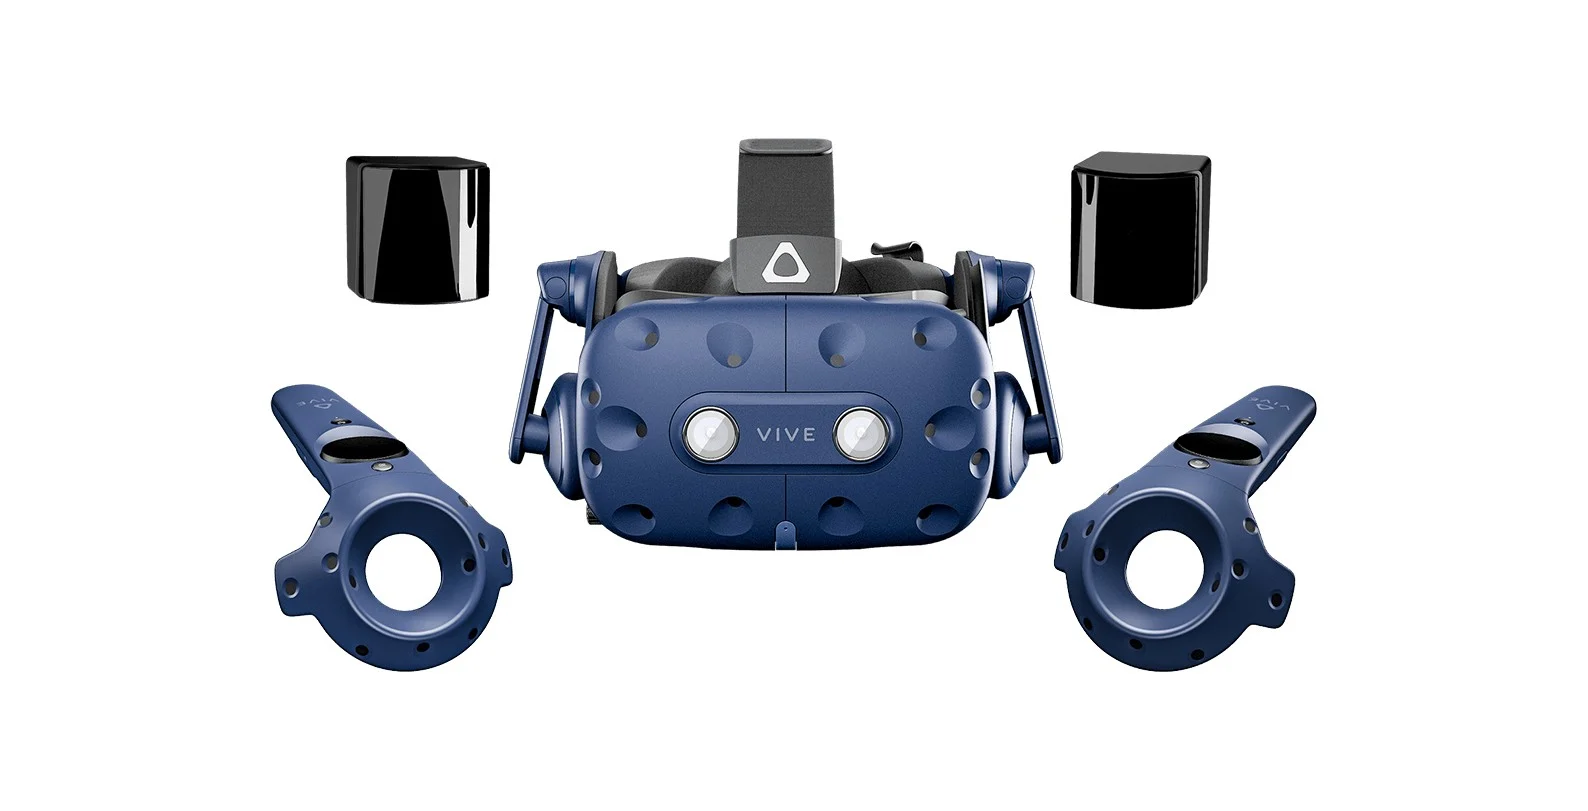
\includegraphics[height=2cm]{images/HtcVice.png} % Altezza uniforme
    \caption{HTC Vive Pro}
    \label{fig:htcvive}
  \end{minipage}
\end{figure}

Essendo una tecnologia in crescita, la realtà virtuale riesce ad attrarre con grande
efficacia l'attenzione dei ragazzi che vedono in essa una rivoluzione nel campo dell'intrattenimento,
che permette di vivere le esperienze di gioco in maniera più coinvolgente, e realistica,
permettendo inoltre interazioni mai viste all'interno di videogiochi
tradizionali. Proprio per questo motivo nasce l'idea di questa tesi che si pone l'obiettivo
di stimolare e al contempo facilitare l'apprendimento degli studenti attraverso strategie
di \textit{gamification} dei contenuti didattici.

\section*{Le applicazioni della realtà virtuale}
\label{sec:le-applicazioni-della-realta-virtuale}

Ad oggi i visori sono usati principalmente per scopo ludico, ma sempre di più si
sta affermando l'uso di questi dispositivi in diversi altri ambiti, come la visualizzazione
di mostre e musei o la simulazione di ambienti di lavoro, e con questo progetto
si vuole applicare questa tecnologia nell'ambito dell'insegnamento della fisica,
una delle materie più complesse che si affrontano nei primi anni delle scuole superiori.

L'applicazione è chiamata \textbf{PhXR} ovvero Physics in eXtended Reality, e consiste
in un laboratorio di fisica virtuale all'interno dei quali gli studenti avranno la
possibilità di sperimentare i concetti fisici visti a lezione in maniera interattiva
e coinvolgente. L'applicazione permette infatti eseguire esperimenti fisici
contenuti in sistemi chiusi nei quali è possibile assumere il completo controllo
di tutte le variabili, permettendo di sperimentare fenomeni impossibili da riprodurre
in un laboratorio reale.

L'idea principale nasce dalla necessità di semplificare l'apprendimento di concetti
teorici difficilmente dimostrabili in un laboratorio reale, come ad esempio la
legge di conservazione dell'energia, o la legge di conservazione della quantità di
moto,che a causa della presenza di agenti esterni non annullabili come la forza d'attrito,
risultano difficili da dimostrare in un laboratorio reale.

Da questa idea il progetto si estende per permettere non solo la semplificazione
di aspetti teorici, ma anche la creazione di nuovi esperimenti che permettano di
visualizzare fenomeni fisici più complessi.

\textbf{TODO: Riferimenti a ricerche che trattano l'uso dei visori nell'insegnamento,
e benefici studiati sull'uso dei visori nell'insegnamento, anche BES}